\documentclass[letterpaper,11pt]{article}
\usepackage[utf8x]{inputenc}
\usepackage[english]{babel}
\usepackage{url}
\usepackage{hyperref}
\usepackage{apacite}
\usepackage{authblk}
\usepackage{booktabs}
\usepackage{tabularx}
\usepackage{caption}
\usepackage{graphicx}
\usepackage[a4paper, total={6.5in,9in}]{geometry}

\captionsetup[table]{labelfont=bf}
\captionsetup[table]{labelsep=period}
\captionsetup[figure]{labelfont=bf}
\captionsetup[figure]{labelsep=period}
\captionsetup[figure]{justification=raggedright,singlelinecheck=false,labelfont=bf}

\usepackage{titlesec}
\titleformat{\section}{\centering\bfseries}{\thesection}{1em}{}
\titleformat{\subsection}{\centering\bfseries}{\thesubsection}{1em}{}
\titleformat{\subsubsection}{\centering\bfseries}{\thesubsubsection}{1em}{}

\title{% 
  \LARGE Psychometrically skewed distributions lead to pseudoclustering when using mixture models: \\ 
   \Large A commentary on “Heterogeneity in children \\ at risk of math learning difficulties” \large (Munez et al., 2023) 
  \ \\
  \ \\
}
\author{Enrico Toffalini}
\affil{Department of General Psychology, University of Padova, Italy}
\renewcommand{\baselinestretch}{1.5} 

\begin{document}
\maketitle
\newpage

\begin{abstract}
Munez et al. (2023) challenge the dimensional framework on learning difficulties by suggesting that children with math difficulties might cluster into qualitatively different types, rather than representing a single homogeneous population. They appropriately employ mixture modeling as the analytical framework of choice. However, the use of non-normally distributed sum scores from mathematical tasks as indicators makes inference problematic. While non-normality is not uncommon in psychological data, it poses a violation of assumptions in the mixture models employed, potentially inflating the number of detected latent classes. Monte Carlo simulations demonstrate that Munez et al. (2023) may have had a heightened likelihood of detecting multiple clusters even in the absence of true latent classes. This case underscores a broader issue in clustering individuals based on psychological data, emphasizing the importance of conducting a priori sanity checks before employing clustering for inference.
\end{abstract}

\newpage

\begin{center} 
\textbf{Psychometrically skewed distributions lead to pseudoclustering when using mixture models: A commentary on “Heterogeneity in children at risk of math learning difficulties” (Munez et al., 2023)}
\end{center}

In a recent study, \citeA{munez2023heterogeneity} challenge the dimensional framework on learning difficulties, suggesting that children with math learning difficulties (MLD) might cluster into two (or even three) qualitatively different types, rather than representing cases of a single homogeneous population. They fit a series of confirmatory factor analyses (CFA), latent profile analyses (LPA), and factor mixture models. The authors appropriately identified mixture models as an ideal method for investigating the existence of subpopulations within a larger set of cases, thus unveiling hidden heterogeneity in what is otherwise traditionally considered an undifferentiated condition. In a similar fashion, in their recent comprehensive review on the “transdiagnostic revolution,” \citeA{astle2022annual} suggested using clustering methods as a primary means of discovering true underlying neurocognitive types beneath the surface of traditional diagnostic categories in neurodevelopmental disorders. While such a data-driven approach should not be used in isolation, \citeA{astle2022annual} present it as a significant complement to the toolbox of the researcher investigating neurodiversity, alongside dimensional methods.

Clustering techniques, including those based on mixture models, rely on certain assumptions to ensure valid statistical inference. Like other statistical methods, even when these assumptions are not met results might still be valid, but their validity is not guaranteed. Many mixture models used in psychology assume multivariate normal distributions. Unfortunately, the normality assumption is generally violated to some degree in our discipline \cite{micceri1989unicorn}. When working on real data the ground truth is unknown, so such risks remain concealed. Luckily, data simulation allows for conducting a priori sanity checks to quantify these risks beforehand. One could simulate data from a known multivariate distribution, with pre-specified features such as correlation, skewness, and kurtosis coefficients. If the chosen clustering method predominantly favors solutions that involve the incorrect number of clusters, this is clearly a problem, and indicates that another method should be used.

\textit{A priori} sanity checks to detect inferential errors via simulation (e.g., \citeNP{toffalini2022entia}) are akin to the famous Monte Carlo simulations generally used for determining power (cf. \citeNP{tein2013statistical} for an example on latent profile analysis). For instance, \citeA{toffalini2022entia} showed that Gaussian mixture models, under a set of specific conditions that may be common in psychological research, tend to incorrectly detect multiple clusters despite data being drawn from a single population. Surprisingly, this occurred even when the distributional assumption was met (i.e., data were generated from perfectly Gaussian multivariate distributions). Such an inflation of detected clusters arose when the sample size was insufficient for modeling the existing covariance across indicators within the detected clusters (e.g., the sample size was medium or even large, but the correlations across multiple indicators were weak). Remarkably, under specific combinations of sample size, correlation coefficients, and number of indicators, it was virtually guaranteed that Gaussian mixture models would detect multiple latent classes/clusters where none existed.

In the case of \citeA{munez2023heterogeneity}, correlations across indicators are quite strong (\textit{r} in [0.52, 0.70]), suggesting that they are likely well modeled using a latent factor. However, violations of assumptions may be a concern here. Sum scores from three mathematical tasks are utilized as indicators. One skewness coefficient is large (0.98 in math fluency), and another is moderately large (-0.68 in numerical operations). Moreover, all kurtosis coefficients are moderately large (absolute values $\geq$ 0.50). 

It is worth noting that skewness in cognitive tasks may simply be a psychometric issue when utilizing sum scores. In \citeA{munez2023heterogeneity}, for example, math fluency has a mean (M) of 14.19 and a standard deviation (\textit{SD}) of 10.34, placing the mean value much closer to the lower (0) than to the upper (48) bound, with it being only 1.37 \textit{SD}s away from the lower bound. To illustrate how sum scores from a binomial distribution may lead to skewness, consider Figure 1. On the left panel, the distribution of \textit{N} = 50,000 simulated cases on a perfectly normal latent trait ("true" z-scores; \textit{M} = 0, \textit{SD} = 1, range in [-$\infty$, +$\infty$]) is shown. On the right panel, the observed distribution of sum scores is displayed. In the simulation, individuals completed a 48-item task with binomial responses. Items were simulated to be moderately difficult on average (\textit{M} = 1, \textit{SD} = 1), resulting in right skewness of scores. The probit function was used to transform latent z-scores into probabilities. The observed sum scores present \textit{M} = 14.24, and \textit{SD} = 9.89, and a skewness coefficient of -0.67. Note that these parameters are quite similar to those reported for math fluency in \citeA{munez2023heterogeneity}, albeit somewhat less skewed. The R code for plotting this figure and the underlying statistical computation is available online at: \url{https://github.com/EnricoToffalini/commentary_mixture_skewness}. 

\begin{figure}[htbp]
	\label{fig:example}
	\caption{\newline \textit{Example of simulated distributions of true latent z-scores and corresponding observed sum scores in 50,000 cases. Dashed vertical lines show the bounds of observed scores.}}
	\centering
	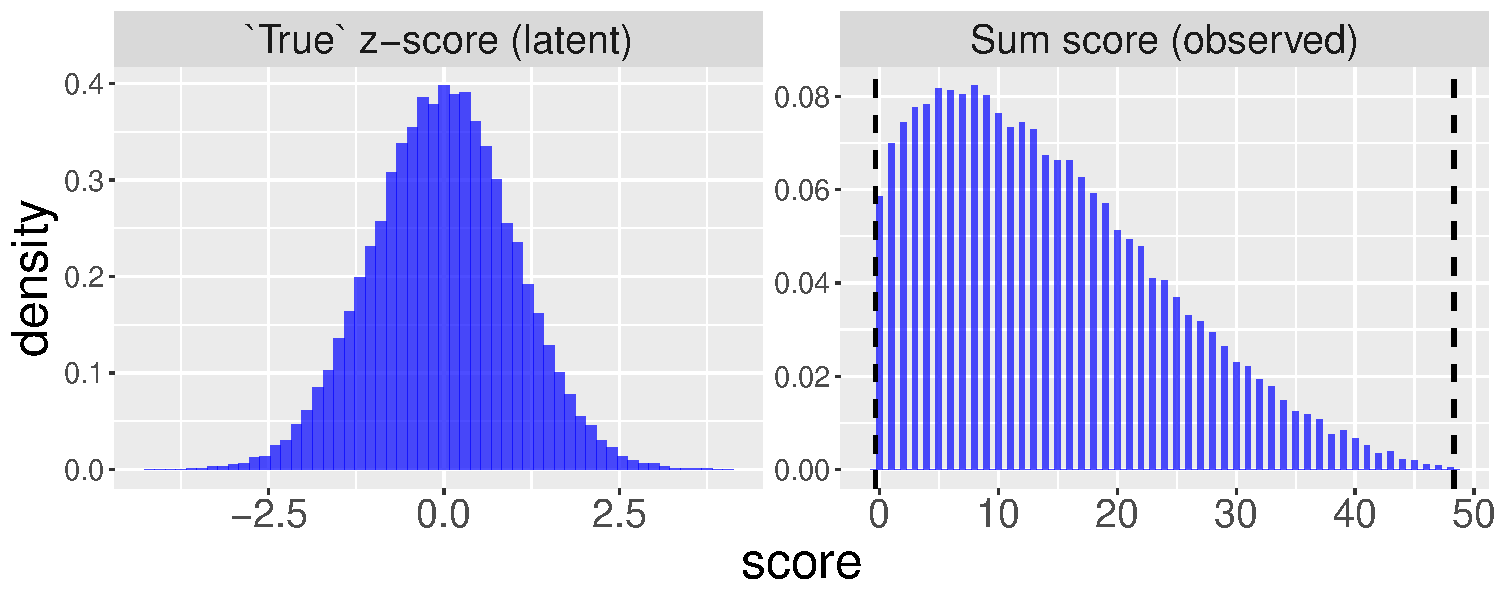
\includegraphics[width=\textwidth]{../R code simulations/z-vs-sumscore.pdf}
\end{figure}

\section*{Data Simulation}

As a retrospective evaluation of the inferential risks in the research scenario presented by \citeA{munez2023heterogeneity}, Monte Carlo simulations were conducted. Data simulation was based on the coefficients reported by the authors in their descriptive statistics table and was executed using the “semTools” package of R, which allows for the simulation of multivariate (non-)normal distributions. The sample size (\textit{N} = 428), correlations, skewness, and kurtosis coefficients for the three measures of math ability used for clustering (i.e., math fluency, math problem solving, and numerical operations) were extracted from the original articles. Commendably, the authors provided the Mplus script that they used for fitting models, which could be reused in the present Monte Carlo simulation analyses. However, as Mplus is licensed, non-open-source software, making it difficult for others to freely replicate the results, additional simplified examples, entirely run with the freely available R software \cite{team2010r} are offered to further clarify the points, and the code is entirely provided.

\section*{Results}

Ten datasets were simulated, and factor mixture models were fitted using the same Mplus code provided by \citeA{munez2023heterogeneity}. Models featuring 1, 2, and 3 latent classes were fitted. Non-invariant model alternatives were preferred both to ensure maximum flexibility and because these were the models chosen by the authors in their final selected solution. In all 10 iterations, BIC consistently favored a three-class solution. The two-class model consistently outperformed the one-class model (median $\Delta$BIC = -134.7), and the three-class model consistently outperformed the two-class model (median $\Delta$BIC = -28.26). In all but one case, the likelihood ratio test also suggested that the one-class hypothesis (H$_{0}$) should be rejected in favor of a two-class solution (\textit{p}s $<$ 0.001), while in five of these cases, the two-class hypothesis (as H$_{0}$) was rejected in favor of the three-class solution (\textit{p}s $<$ 0.05). Results are presented in Table 1.

\begin{table}[htbp]
    \centering
    \label{tab:iterationResults}
    \caption{\newline \textit{Results from 10 iterations of running factor mixture model, 1-3 classes, on simulated data with 3 indicators and parameters taken from Munez et al. (2023). Data present significant skewness and kurtosis (see text). There are no true latent classes, but the BIC consistently and correctly favors the 3-class solution. N = 428.}}
    \begin{tabularx}{\textwidth}{XXXXXX}
       \toprule
        \textbf{Iteration} & \textbf{BIC \newline(1 class)} & \textbf{BIC \newline(2 classes)} & \textbf{BIC \newline(3 classes)} & \textbf{LRT p-val \newline(2 vs 1 cl.)} & \textbf{LRT p-val \newline(3 vs 2 cl.)}  \\
        \midrule
        1 & 3260.71 & 3117.46 & 3058.55 & \textless 0.001 & \textless 0.001 \\
        2 & 3231.70 & 3120.85 & 3102.48 & \textless 0.001 & 0.002 \\
        3 & 3244.15 & 3101.92 & 3062.66 & \textless 0.001 & \textless 0.001 \\
        4 & 3123.03 & 2999.45 & 2979.78 & \textless 0.001 & 0.005 \\
        5 & 3189.74 & 3050.75 & 3022.55 & \textless 0.001 & 0.275 \\
        6 & 3164.93 & 3035.99 & 3011.98 & \textless 0.001 & 0.052 \\
        7 & 3228.02 & 3051.49 & 3048.14 & \textless 0.001 & 0.076 \\
        8 & 3131.17 & 2978.36 & 2931.72 & \textless 0.001 & \textless 0.001 \\
        9 & 3140.58 & 3024.68 & 2996.36 & 0.113 & 0.010 \\
       10 & 3199.68 & 3069.27 & 3016.92 & \textless 0.001 & 0.055 \\
        \bottomrule
    \end{tabularx}
\end{table}

As a further sanity check, all 10 datasets were re-simulated with perfectly normal distributions (i.e., with all skewness and kurtosis coefficients set to zero in the data-generating process). In this second case, the BIC consistently (and correctly) favored the one-class solution (median $\Delta$BIC = +17.94 in favor of the one-class over the two-class solution, and median $\Delta$BIC = +19.50 in favor of the two-class over the three-class solution). Results are presented in Table 2. This double check confirmed that the inflation of the number of detected clusters was due to non-normality. Caution should be used, however, as several warnings emerged indicating that the latent variable covariance matrix was not positive definite in one or more classes, especially with the three-class solutions.

\begin{table}[htbp]
    \centering
    \label{tab:iterationResults}
    \caption{\newline \textit{Results from 10 iterations of running factor mixture model, 1-3 classes, on simulated data with 3 indicators and correlations taken from Munez et al. (2023), but without any skewness and kurtosis (all parameters were fixed to zero). There are no true latent classes, and the BIC consistently favors the 1-class solution. N = 428.}}
    \begin{tabularx}{\textwidth}{XXXXXX}
       \toprule
        \textbf{Iteration} & \textbf{BIC \newline(1 class)} & \textbf{BIC \newline(2 classes)} & \textbf{BIC \newline(3 classes)} & \textbf{LRT p-val \newline(2 vs 1 cl.)} & \textbf{LRT p-val \newline(3 vs 2 cl.)}  \\
        \midrule
        1 & 3143.40 & 3170.59 & 3184.05 &  0.408 & \textless 0.001 \\
        2 & 3138.86 & 3144.23 & 3161.86 &  0.013 & 0.011 \\
        3 & 3219.51 & 3239.62 & 3266.04 &  0.603 & \textless 0.001 \\
        4 & 3242.65 & 3261.33 & 3285.14 &  0.379 & 0.256 \\
        5 & 3170.24 & 3188.30 & 3216.56 &  0.074 & \textless 0.001 \\
        6 & 3165.85 & 3180.07 & 3199.54 &  0.087 & \textless 0.001 \\
        7 & 3180.55 & 3203.14 & 3222.67 &  0.443 & 0.025 \\
        8 & 3194.90 & 3212.72 & 3241.66 &  0.059 & 0.373 \\
        9 & 3180.20 & 3187.64 & 3193.73 & 0.036 & 0.139 \\
       10 & 3184.38 & 3199.03 & 3217.02 &  0.007 & 0.093 \\
        \bottomrule
    \end{tabularx}
\end{table}


\titleformat{\subsection}[hang]{\normalfont\bfseries}{\thesubsection}{1em}{}
\subsection*{Additional analyses}

For further clarification, additional Monte Carlo simulations of Gaussian mixture models were conducted in R. The code is provided on GitHub at \url{https://github.com/EnricoToffalini/commentary_mixture_skewness}. The well-known “mclust” package \cite{scrucca2016mclust} was utilized. Tested solutions featured 1 to 3 components (latent classes/clusters), with BIC serving as the criterion for determining the optimal solution. Initially, 1,000 iterations were executed, simulating datasets each with \textit{N} = 428, featuring skewness and kurtosis as reported above. Notably, in all cases, data were drawn from a single population, with no true clusters present. Despite this, the one-class solution was never favored by the BIC, despite being the correct one. In 41.4\% of iterations, the two-class solution was favored, and in the remaining 58.6\% of iterations, the three-class solution was favored. Subsequently, another 1,000 iterations were run. In this set, the same \textit{N} and correlations across variables were simulated, but all skewness and kurtosis coefficients were set to zero. In this case, the one-class solution was (correctly) selected as optimal in 100\% of iterations. This suggests that skewness and kurtosis are indeed the underlying factors contributing to the inflated number of latent classes detected.

\section*{Discussion}

The results suggest that there may not be evidence of hidden heterogeneity in children with MLD, while the previous report of multiple clusters may reflect a statistical artifact. While the ground truth of the data-generating process remains unknown concerning the real data, the present Monte Carlo simulation demonstrates that \citeA{munez2023heterogeneity} had a very high chance of detecting multiple clusters even if no true latent classes existed within MLD. This article takes the opportunity to highlight a larger problem regarding clustering individuals based on psychological data. The main issue, in this case, appears to be the data not meeting the normality assumption. As explained earlier, non-normality may simply reflect the characteristics of the tasks used, and it is a widespread problem in psychometrics (e.g., \citeNP{micceri1989unicorn}). When assessing achievement or cognitive abilities in developmental samples, sum scores are often computed. As previously shown in Figure 1, sums of binomial (correct/incorrect) responses may lead to skewness. This is generally true unless the distribution averages around 50\%, and in any case, its mean and \textit{SD} are non-independent (e.g., \citeNP{edwards1960meaning}). To address this issue, researchers might consider dropping sum scores and using estimates of individual ability drawn from models adequate for dealing with binomial responses, such as those based on Item Response Theory (IRT), or predicted scores preliminarily obtained from Confirmatory Factor Analysis (CFA) with ordinal items; these may be preferred solutions for normalizing scores.

Another challenge is that for true clusters to be correctly detected, their separation across clustering indicators must be sufficiently large. \citeA{tein2013statistical} suggest that separations should be at least Cohen’s \textit{d} = 0.8 on several independent dimensions for clusters to emerge in latent profile analysis, and similar conclusions were reached by \citeA{toffalini2022entia} for Gaussian mixture models. Such large effect sizes on many orthogonal variables may generally seem implausible in psychological research, and they are certainly unlikely to have remained undetected until data-driven exploratory research was conducted. Effect sizes with a magnitude larger than 1.0 standardized mean difference can be considered "very large" in psychology \cite{funder2019evaluating}, raising suspicions when they emerge seemingly "randomly" in exploratory research on individual differences. In \citeA{munez2023heterogeneity}, the separations between the two detected clusters are quite substantial: the intercepts differ by more than 1.0 \textit{SD} in all three indicators of math ability, and several other domain-general and domain-specific cognitive variables exhibit between-cluster mean differences close to 1.0 \textit{SD}. Additionally, the fact that one cluster outperforms the other(s) in all variables simultaneously might also indicate an inflation in the number of detected latent classes \cite{toffalini2022entia}.

The problem of the large separation required across clusters is particularly critical as clusters emerging via data-driven methods cannot easily be corroborated by other sources of evidence. It is worth noting that, unlike correlations or mean differences, no descriptive statistics or data visualization can back up inference unless visual inspection of scatter plots clearly suggests multimodal distributions. Unfortunately, multimodal distributions are unlikely to emerge in psychological research on individual differences, as they would require very large effect sizes. To clarify, distributions that are separated by more than 1.0 \textit{SD} (i.e., Cohen’s \textit{d}s $\gg$ 1.0) are required for observing multimodality in data distributions (e.g., \citeNP{murphy1964one}). The issue is illustrated in Figure 2. \textit{N} = 10,000 normally-distributed, bivariate observations are generated. Bivariate multimodality is barely visible despite very large separation (Euclidean distance is \textit{D} = 2.83), while univariate multimodality fails to emerge despite Cohen's \textit{d} = 2.0 in either dimension. 

\begin{figure}[htbp]
	\label{fig:example}
	\caption{\newline \textit{Scatter plot and univariate and bivariate density plots of two clusters separated d = 2.0 on two different, orthogonal dimensions.}}
	\centering
	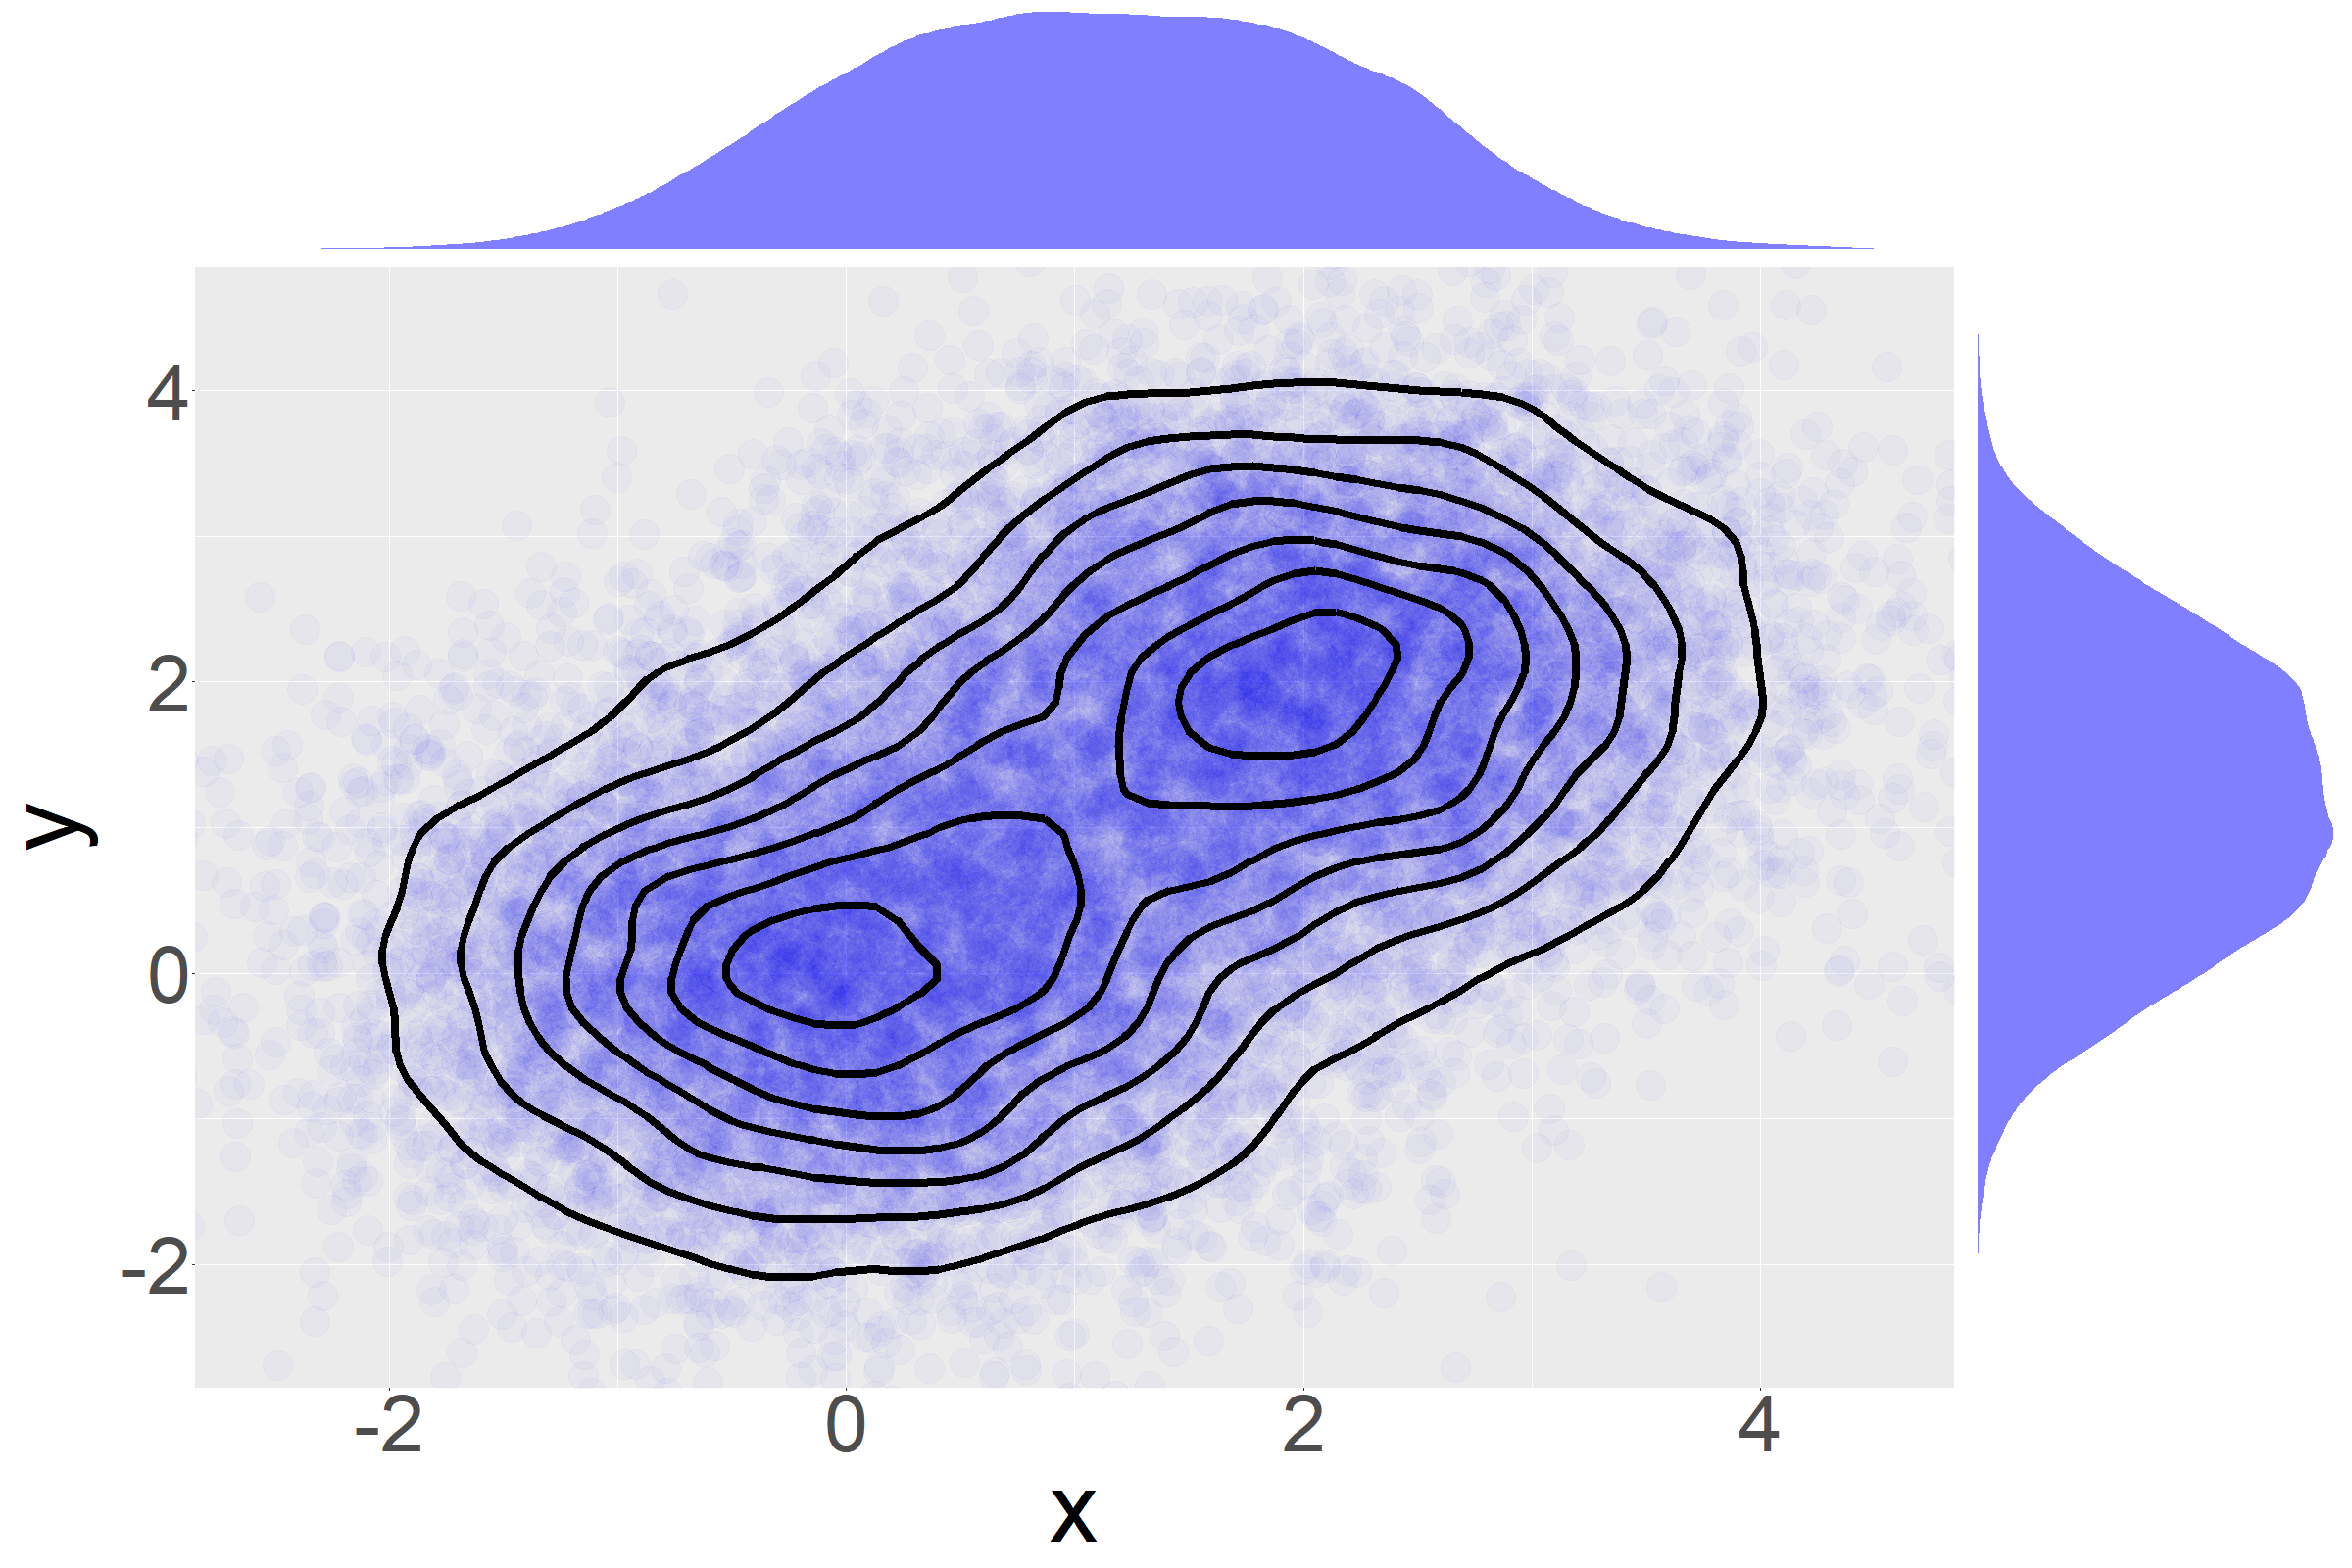
\includegraphics[width=\textwidth]{../R code simulations/biviariate-scatter-plot.png}
\end{figure}

Moving forward, it is crucial to approach clustering techniques with caution in psychological research, especially when inference is the goal. When uncertain, a researcher may run Monte Carlo simulations as a good \textit{a priori} sanity check to see if the chosen clustering methods provide valid results when the ground truth is known, considering the characteristics of the data. An example of R code has been provided for this purpose. In addition to quantifying a “\textit{type I} error of clustering”, that is the risk of detecting multiple classes when in fact only one exist, the readers may also want to quantify statistical power, which is the probability of detecting the correct number of classes when true clusters/latent classes exist \cite{tein2013statistical}.  However, as shown by simulation studies (e.g., \citeNP{tein2013statistical}), sufficient power requires effect sizes of about Cohen’s \textit{d} = 0.80 or above in many independent dimensions simultaneously, which borders on credibility in psychology.
\\
\\
\subsection*{Code and data availability }
Code and data used in this article are fully available on GitHub at: \url{https://github.com/EnricoToffalini/commentary_mixture_skewness}
\newpage
\bibliographystyle{apacite}
\bibliography{references.tex}
\end{document}





